\documentclass[aspectratio=169]{beamer}

% ---------- ENCODING & FONTS ----------
\usepackage[utf8]{inputenc}
\usepackage[T1]{fontenc}

% ---------- THEME & LOOK ----------
\usetheme{Madrid}
\usecolortheme{seahorse}
\usefonttheme{professionalfonts}
\setbeamertemplate{navigation symbols}{}
\setbeamercovered{transparent}
\setbeamertemplate{itemize items}[circle]
\setbeamertemplate{enumerate items}[default]
\setlength{\parskip}{0.25em}

% ---------- COLORS ----------
\usepackage{xcolor}
\definecolor{accent}{RGB}{0,92,184}
\definecolor{soft}{RGB}{233,244,255}
\setbeamercolor{structure}{fg=accent}
\setbeamercolor{title}{fg=white,bg=accent}
\setbeamercolor{frametitle}{fg=accent}
\setbeamercolor{block title}{bg=accent!12,fg=accent}
\setbeamercolor{block body}{bg=soft}

% ---------- PACKAGES ----------
\usepackage{booktabs}
\usepackage{amsmath, amssymb}
\usepackage{array}
\usepackage{multirow}
\usepackage{hyperref}
\hypersetup{colorlinks=true,linkcolor=accent,urlcolor=accent}

% ---------- SAFE FALLBACK FOR TRANSITIONS ----------
\makeatletter
\@ifundefined{transfade}{\newcommand{\transfade}[1][]{}}{}
\makeatother

% ---------- PLACEHOLDER BOX (compile-safe; no images required) ----------
\newcommand{\placeholderbox}[2][0.82\linewidth]{%
  \begin{center}
    \fbox{\begin{minipage}[c][0.46\textheight][c]{#1}
      \centering \vspace{0.25em}
      \textbf{#2}\\[0.6em]
      \emph{Insert figure/diagram here later.}
    \end{minipage}}
  \end{center}
}

% ---------- TITLE ----------
\title{\textbf{Unemployment: Causes and Consequences  \vspace{.5cm}\\  }}
\subtitle{ {\large ECON 300 - Labour Economics}}
%\institute{UNBC}
\author{Muhebullah Karimzada}

\date{Winter 2026}


\begin{document}

% ============================================================
% TITLE
% ============================================================
\begin{frame}[plain]
  \titlepage

\end{frame}

% ============================================================
\section{Learning Objectives \& Main Questions}
% ============================================================

\begin{frame}{Learning Objectives (1/2)}
\transfade
\begin{itemize}[<+->]
  \item Explain how imperfect information yields coexistence of unemployment and vacancies.
  \item Assess how technological change (esp.\ the Internet) affects job search/matching.
  \item Show how demand shifts and sectoral change can generate unemployment.
  \item Summarize evidence on job displacement and consequences.
\end{itemize}
\end{frame}

\begin{frame}{Learning Objectives (2/2)}
\transfade
\begin{itemize}[<+->]
  \item Describe models where firms pay above-market wages (efficiency wages, contracts, insider--outsider).
  \item Explain the rationale for unemployment insurance and its effects on labour supply and unemployment.
  \item Summarize empirical evidence on UI/EI, incidence, and duration of unemployment.
\end{itemize}
\end{frame}

\begin{frame}{Main Questions}
\transfade
\begin{itemize}[<+->]
  \item What role does \alert{wage rigidity} play in unemployment?
  \item How does \alert{imperfect information} create frictional unemployment?
  \item Is online search improving matching efficiency?
  \item What are the consequences of job loss for workers and families?
  \item Does UI/EI do more harm than good?
\end{itemize}
\end{frame}

% ============================================================
\section{Causes of Unemployment}
% ============================================================

\begin{frame}{Causes of Unemployment}
\transfade
\begin{itemize}[<+->]
  \item Minimum wage laws
  \item Institutional factors (unions, large public sector)
  \item Demand factors \& seasonal unemployment
  \item \textbf{Frictional} unemployment from normal turnover \& imperfect info
  \item \textbf{Sectoral shifts} causing structural unemployment (time-to-match)
  \item \textbf{Generous UI/EI} affecting search incentives
\end{itemize}
\end{frame}

% ============================================================
\section{Frictional vs.\ Structural: Job Search}
% ============================================================

\begin{frame}{Search Unemployment: Core Ideas}
\transfade
\begin{itemize}[<+->]
  \item Imperfect information delays matching; search has costs and benefits.
  \item \textbf{Stopping rule (reservation criteria):} set minimum acceptable wage/conditions; accept first offer meeting it.
  \item Optimal search balances \alert{expected marginal benefit} and \alert{expected marginal cost}.
\end{itemize}
\end{frame}

\begin{frame}{Figure 17.1: Optimal Job Search }
\vspace{.2cm}
\centering
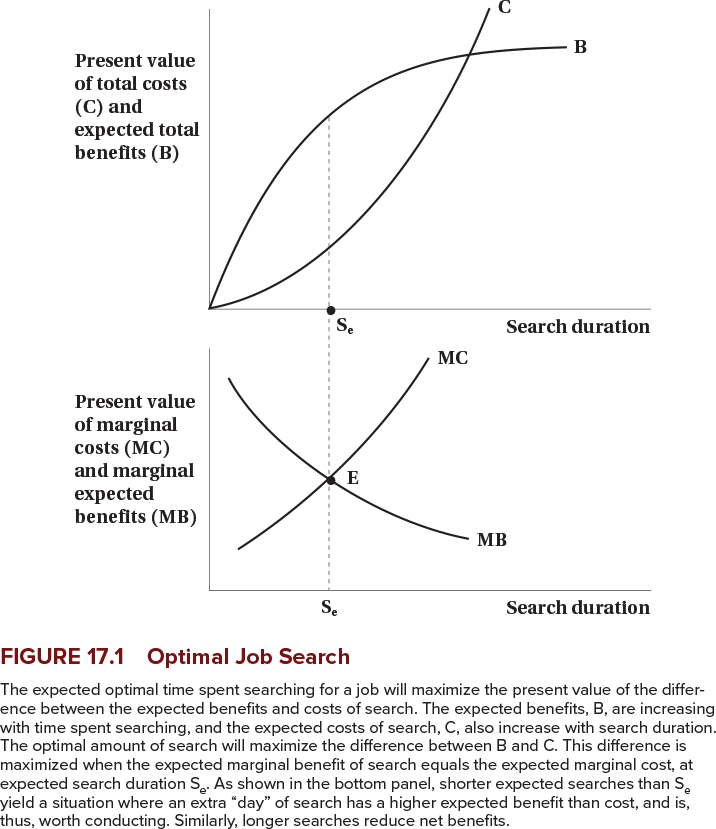
\includegraphics[width=0.55\linewidth]{ben54842_1701}
\end{frame}

\begin{frame}{Imperfect Information: Market Implications}
\transfade
\begin{itemize}[<+->]
  \item Markets do not clear instantaneously.
  \item \textbf{Wage dispersion} persists even with homogeneous workers/jobs.
  \item “Dynamic monopsony” features: individual firms face upward-sloping supply due to frictions.
\end{itemize}
\end{frame}

\begin{frame}{Figure 17.2: Wage Distributions Under Imperfect vs.\ Perfect Information }
\centering
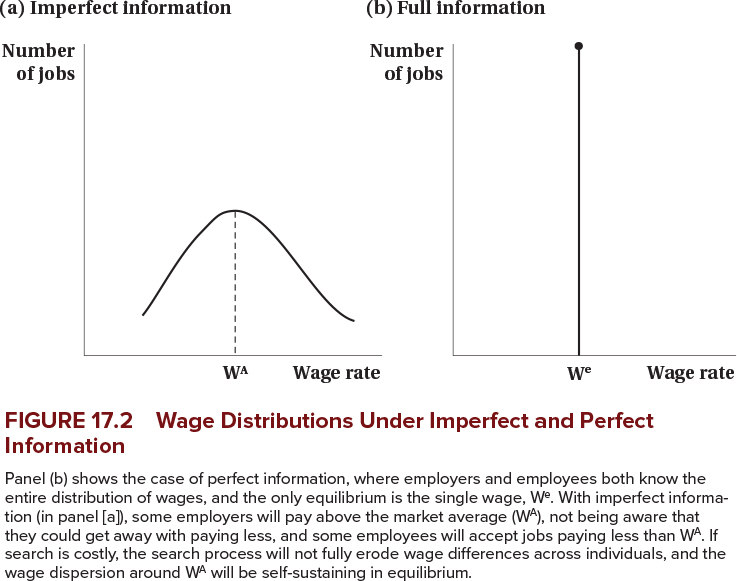
\includegraphics[width=0.89\linewidth]{ben54842_1702}
\end{frame}

\begin{frame}{Worked Example: Reservation Wage and Hazard}
\transfade
\small
Julia faces three job types with equal probability: \$2{,}400, \$2{,}200, \$2{,}000 per month.\par
\begin{itemize}[<+->]
  \item Expected value of next offer: \(\mathbb{E}[W]=\$2{,}200\).
  \item \textbf{Reservation wage:} Julia rejects any offer \(< \$2{,}200\) and accepts the first \(\ge\$2{,}200\).
  \item \textbf{Hazard (acceptance) probability:} \(P(W\ge 2{,}200)=2/3\).
  \item Intuition: Higher search cost \(\Rightarrow\) lower reservation wage; better offer distribution \(\Rightarrow\) higher reservation wage.
\end{itemize}
\end{frame}

\begin{frame}{Determinants of Optimal Search — \textit{Placeholder for Diagram}}
\transfade
\placeholderbox{Factors Determining Optimal Search — Map costs (benefits foregone) vs.\ expected gains; show shifts in $S_e$.}
\end{frame}

% ============================================================
\section{Evidence on Job Search}
% ============================================================

\begin{frame}{Table 17.1: Search Activity of the Unemployed, 2019}
\transfade
\scriptsize
\begin{tabular}{lcc}
\toprule
\textbf{Group and Search Activity} & \textbf{Number Using Activity (thousands)} & \textbf{Percent Using Activity (\%)} \\
\midrule
Unemployed: Did not search & 101 & 8.8 \\
Unemployed: Searched for full-time work & 747 & 65.3 \\
Unemployed: Searched for part-time work & 295 & 25.8 \\
Search activity: Looked at advertisements & 684 & 59.8 \\
\quad Contacted employers directly & 441 & 38.6 \\
\quad Placed or answered advertisements & 402 & 35.2 \\
\quad Checked with friends or relatives & 265 & 23.2 \\
\quad Used public employment agency & 134 & 11.7 \\
\quad Used private employment agency & 84 & 7.4 \\
\bottomrule
\end{tabular}
\end{frame}

\begin{frame}{Search, the Internet, and Matching}
\transfade
\begin{itemize}[<+->]
  \item Rapid growth in online job boards, employer portals, and screening tools.
  \item Formal search models increasingly estimated with micro data.
  \item \textbf{Mechanism:} Tech can raise contact rates and shorten time-to-fill; screening may raise match quality.
\end{itemize}
\end{frame}

% ============================================================
\section{Sectoral Shifts \& Displacement}
% ============================================================

\begin{frame}{Sectoral Shifts and Unemployment}
\transfade
\begin{itemize}[<+->]
  \item Major structural change raises unemployment during reallocation.
  \item Highly cyclical industries amplify unemployment in downturns.
  \item Regional reallocation in Canada drives relocation and search.
\end{itemize}
\end{frame}

\begin{frame}{Figure 17.3: Regional Unemployment Rates, 1976--2019}
\centering
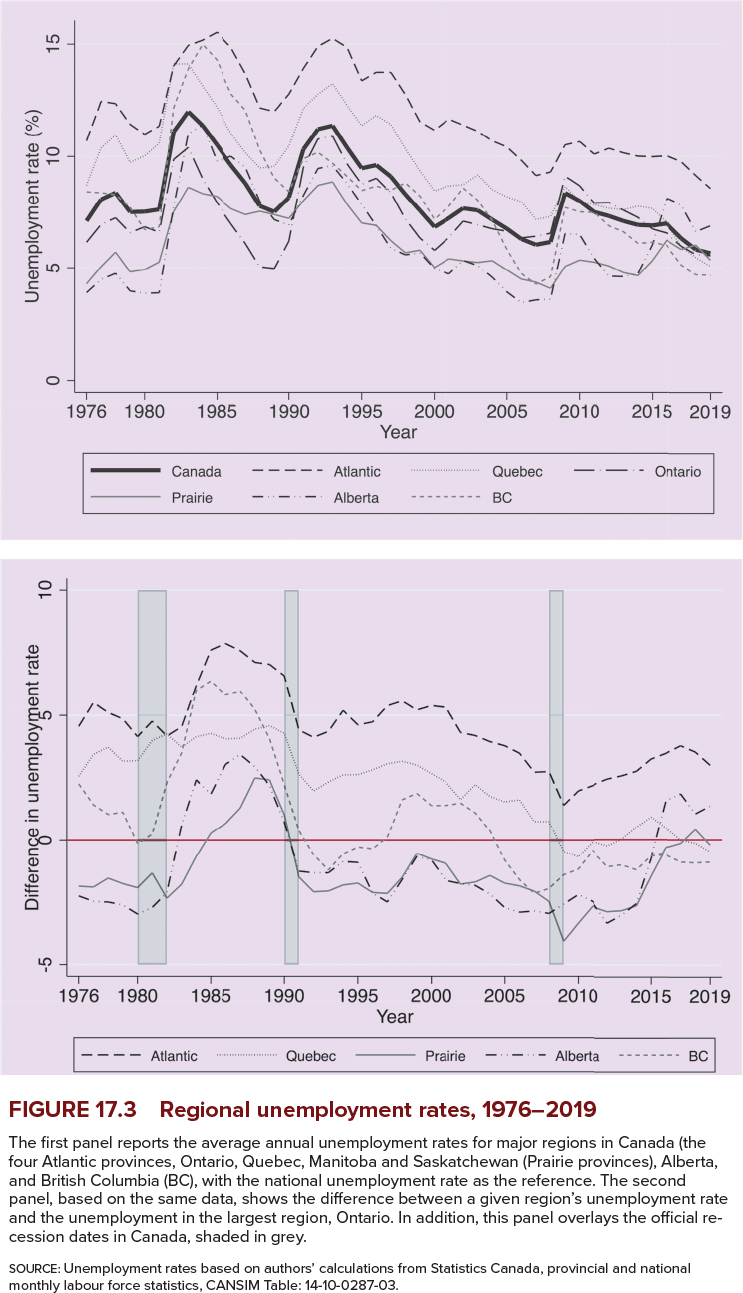
\includegraphics[width=0.34\linewidth]{ben54842_1703}
\end{frame}

\begin{frame}{Displaced Workers: Stylized Findings}
\transfade
\begin{itemize}[<+->]
  \item Permanent job loss yields \alert{large earnings losses}, esp.\ after stable attachments.
  \item Re-employment often at substantially lower wages; losses can be long-lasting.
  \item Older and less-educated workers have lower re-employment probabilities.
\end{itemize}
\end{frame}

% ============================================================
\section{High-Wage Unemployment: Above-Market Pay}
% ============================================================

\begin{frame}{Three Approaches}
\transfade
\begin{itemize}[<+->]
  \item \textbf{Implicit contracts} (risk sharing; rigid wages; layoffs in bad states)
  \item \textbf{Efficiency wages} (morale, shirking, turnover, union avoidance, nutrition)
  \item \textbf{Insider--outsider} (incumbents bargain; outsiders have little influence)
\end{itemize}
\end{frame}

\begin{frame}{Implicit Contracts: Risk Sharing}
\transfade
\begin{itemize}[<+->]
  \item Workers are typically more risk-averse (human capital not diversifiable).
  \item Contracts stabilize income with a \alert{rigid wage} \(W^\ast\); employment adjusts across states.
  \item Good state: \(N_0,\, W^\ast\) below spot wage; Bad state: \(N_b^\ast > N_b,\, W^\ast\) above spot wage.
\end{itemize}
\end{frame}

\begin{frame}{Figure 17.4: Implicit Contracts }
\centering
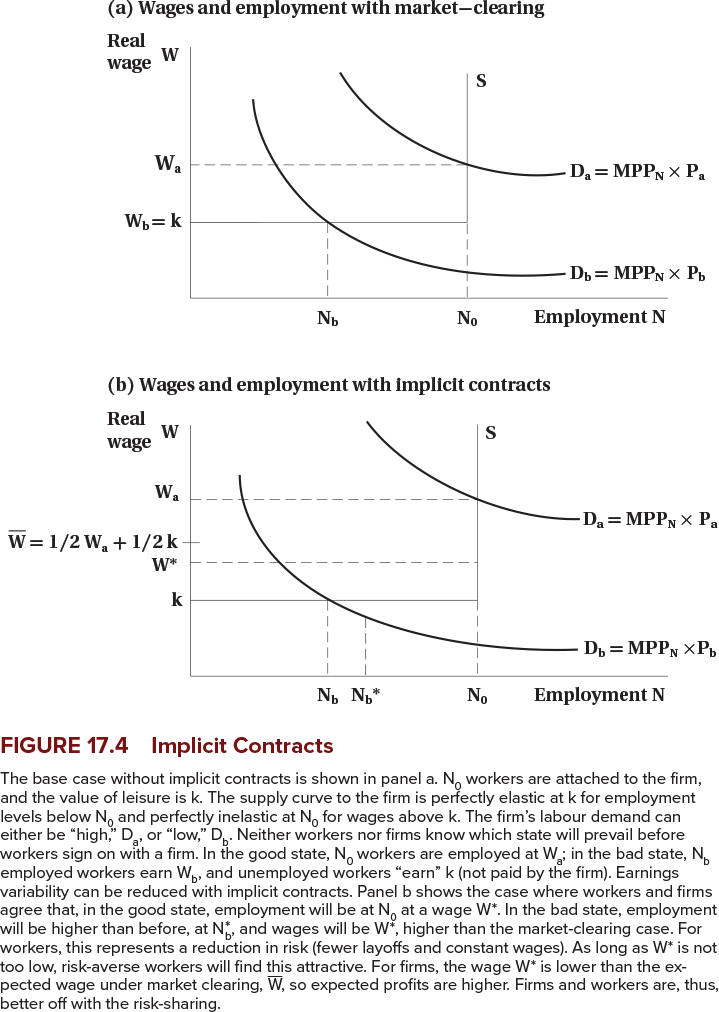
\includegraphics[width=0.485\linewidth]{ben54842_1704}
\end{frame}

\begin{frame}{Efficiency Wages: Core Mechanisms}
\transfade
\begin{itemize}[<+->]
  \item Higher wages can raise effort/morale, reduce shirking/turnover, and deter unionization.
  \item \textbf{Nutritional model:} Efficiency $e(W)$ rises with $W$ up to threshold; diminishing returns after.
\end{itemize}
\end{frame}

\begin{frame}{Figure 17.5: Determination of the Efficiency Wage }
\centering
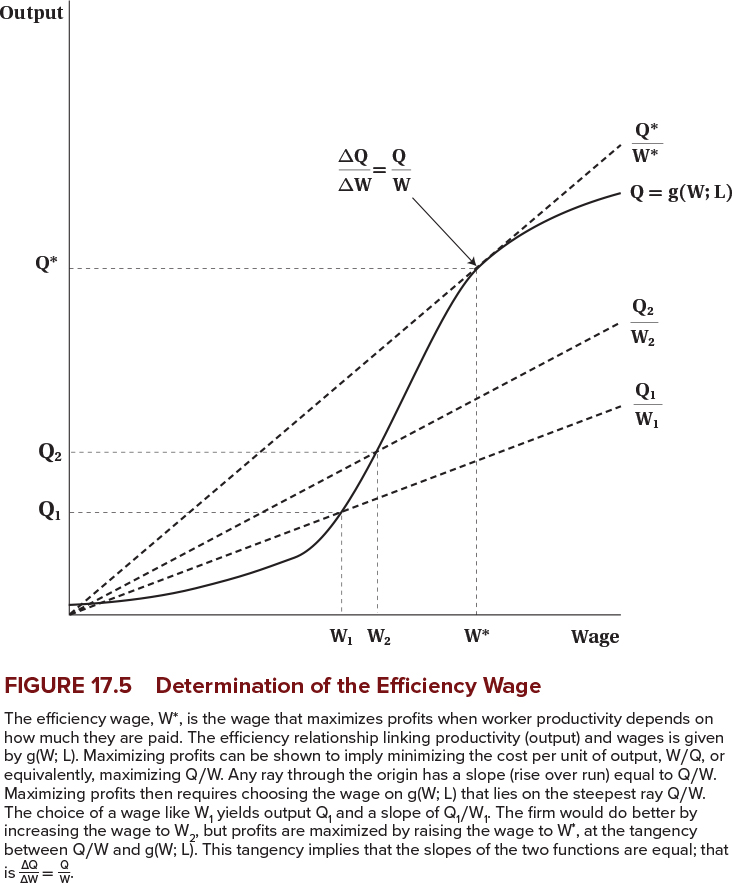
\includegraphics[width=0.55\linewidth]{ben54842_1705}
\end{frame}

\begin{frame}{Insider--Outsider Theory}
\transfade
\begin{itemize}[<+->]
  \item Wages are bargained with incumbents; replacement of insiders is costly.
  \item Excess supply (outsiders) exerts limited pressure on wages.
  \item Result: Wage rigidity and persistent unemployment.
\end{itemize}
\end{frame}

% ============================================================
\section{Unemployment Insurance (UI/EI)}
% ============================================================

\begin{frame}{Economic Rationale for UI/EI}
\transfade
\begin{itemize}[<+->]
  \item Insurance against income loss from unemployment.
  \item Alters \textbf{incidence} (job separations) and \textbf{duration} (search length) via incentives and liquidity.
\end{itemize}
\end{frame}

\begin{frame}{Channels: Incidence and Duration}
\transfade
\begin{itemize}[<+->]
  \item Higher benefits raise the value of search for employed \(\Rightarrow\) may increase separations.
  \item For unemployed, benefits lower search costs \(\Rightarrow\) longer optimal search.
  \item Empirically, exit hazards often \alert{spike at benefit exhaustion}.
\end{itemize}
\end{frame}

\begin{frame}{Canada’s UI/EI System: Key Features}
\transfade
\begin{itemize}[<+->]
  \item Established 1940; major reforms 1971--72; renamed EI in 1996; refinements in 2000.
  \item \textbf{Replacement rate:} 55\% for beneficiaries.
  \item Hours-credit rules historically allowed similar eligibility from 15 vs.\ 50 hours/week (policy details evolved).
  \item \textbf{Claimant types:} Frequent, Long-tenured, Occasional.
\end{itemize}
\end{frame}

\begin{frame}{Behavioural Effects and Design Considerations}
\transfade
\begin{itemize}[<+->]
  \item Moral hazard vs.\ liquidity effects; durations depend on prior work experience.
  \item Repeat use; regional extended benefits; participation impacts.
  \item \textbf{Design goal:} Balance social insurance value against induced unemployment.
\end{itemize}
\end{frame}

% ============================================================
\section{Chapter Summary}
% ============================================================

\begin{frame}{Summary}
\transfade
\begin{itemize}[<+->]
  \item Wage rigidity and imperfect information explain unemployment with vacancies.
  \item Search theory: reservation wages and hazard rates organize decisions.
  \item Sectoral shifts and displacement generate significant, persistent earnings losses.
  \item Above-market pay arises via contracts, efficiency wages, and insider--outsider forces.
  \item UI/EI provides insurance but shapes incidence and duration; careful design is essential.
\end{itemize}
\end{frame}

\begin{frame}
\centering
\Huge{\textbf{Thank You!}} \\

\end{frame}

\end{document}
